\graphicspath{{chapters/notes/08/images/}}
\chapter{Liquid biopsies in oncology}

\section{Introduction}

    \subsection{Tracking tumour progression}
    It is more feasible to track the tumour progression stage for a patient from liquid biopsies rather than from tissue biopsies.
    Liquid biopsies give a panoramic overview at a particular time point of patient's state, while tissue biopsies an highly accurate snapshot in a specific site at a particular time point.
    This is because liquid biopsies are minimally invasive, allowing to collect more time points.
    Furthermore it is easier for early diagnostics or screening and to quantify the presence of minimal residues of diseases.
    However the accuracy of a liquid biopsy depends on many factors.
    In particular, an homogeneous sample is able to achieve similar quality to the one from a tissue biopsy.

    \subsection{Differences between tissue and liquid biopsies}
    The main difference between tissue and liquid biopsies are listed in table \ref{tab:diff1}.

    \begin{table}[H]
        \centering
        \begin{tabular}{ | p{4cm} | p{9cm} | }
             \hline
             Tissue Biopsy & Liquid Biopsy \\
             \hline
             Accurate and detailed view of one tissue only. & Landscape overview, with resolution depending on tumour burden, releasing rates, metastases and tumour heterogeneity. It is possible to get an aggregated signal of different tumour cell populations. \\
             \hline
             Single tumour. & Possibility of getting signal from multiple tumour masses.\\
             \hline
             Signal relative to a specific point in time. & Signal relative to different specifics point in time obtained through longitudinal sampling.\\
             \hline
             Invasive and painful for the patient, not feasible for all the tissues or in presence of metastatic sites. & Minimally invasive, it can be coupled with a routine blood draw, allowing to collect samples multiple times.\\
             \hline
        \end{tabular}
        \caption{Main differences between tissue and liquid biopsy.}
        \label{tab:diff1}
    \end{table}

        \subsubsection{Liquid biopsies allow to perform a number of analysis}
        Moreover liquid biopsies allow to perform data analysis otherwise impossible with tissue biopsies:

        \begin{multicols}{2}
            \begin{itemize}
                 \item Specific assays can be designed to detect minimal quantities of tumour cells. This is useful to detect minimal residual disease (MRD) that can remain after surgery and avoid tumour recurrence.
                 \item The collection of serial samples allows to:

                     \begin{itemize}
                         \item Track clonal evolution of the tumour over time.
                         \item Catch treatment resistances early on.
                         \item Monitor the patient's response to the treatment.
                     \end{itemize}

                 \item It can be used for early detection of cancer.
             \end{itemize}
         \end{multicols}

         \subsubsection{Material availability}
         Samples obtained through tissue biopsy come from:

         \begin{multicols}{2}
             \begin{itemize}
                 \item Needle biopsies.
                 \item Biopsies.
                 \item Surgical resection (if some material is left after the clinical protocol and the patient agrees to a research protocol).
             \end{itemize}
         \end{multicols}

         Samples obtained through liquid biopsies come from:

         \begin{multicols}{2}
             \begin{itemize}
                 \item Circulating tumour cells.
                 \item Extracellular vescicles.
                 \item Cell-free DNA.
             \end{itemize}
         \end{multicols}

         In particular considering cell-free DNA a difference in its concentration in a sample is visible from a healthy and tumour sample.
         In particular for healthy donor it has a concentration of $\sim 4\frac{ng}{ml}$ and belo $10\frac{ng}{ml}$.
         In tumour patients the range of this concentration varies more and can reach $\sim 100\frac{ng}{ml}$.
         This concentration tends to increase as the tumour becomes metastatic.
         Another factor that influences cel-free DNA concentration is treatment: tumour patients under treatment tend to have a concentration of cfDNA similar to healthy individuals.
         cfDNA concentration is influenced by a lot of factors, making it impossible to use it as a good prognostic feature by itself.

         \subsubsection{Tumour content}
         Tumour content in tissue biopsies can be assessed through a visualization protocol: the proportion of tumour cells compared to healthy one is measured counting the cell in the sample.
         Tumour and healthy cells are distinguished through staining or through their differences in morphology.
         Concentration is computed considering the magnification of the image.
         Subtyping is performed through a staining for biomarkers.
         Also some computational methods are available.
         Instead, for liquid biopsies the fraction of circulating tumour DNA or ctDNA is inferred with methods based on genomics or on methylomics.

         \subsubsection{Assessment of tumour ploidy}
         For tissue biopsies tumour ploidy is assessed through:

         \begin{multicols}{3}
             \begin{itemize}
                 \item Cytogenetics.
                 \item FISH.
                 \item NGS data.
             \end{itemize}
         \end{multicols}

         The average ploidy of samples from liquid biopsies is inferred computationally based on a genomic process, but it is difficult to reach significative results.

    \subsection{Application-dependent requirements}

        \subsubsection{Early tumour, MRD and recurrence detection}
        When performing early tumour detection minimal residual detection and recurrence detection tumour quantity is low.
        So a low signal is expected and an higher quantity of starting higher material is required.
        The quantity to be used need to be finely tuned to balance false positives, which arise from too much material and false negatives, which arise from too little material.

        \subsubsection{Analysis of tumour dynamics, treatment response and analysis of the mechanisms of resistance}
        When performing analysis of tumour dynamics, treatment response and analysis of the mechanisms of resistance the assay should be designed in order to be able to distinguish between different clones.
        So a subclonality analysis should be possible.

        \subsubsection{Single biomarker assessment}
        When performing biomarker assessment the only important thing to take into consideration is to detect whether one point mutation is present or not.
        In this case tumour content is not important.
        A target assay is used and specific locations associated with the SNV are sequenced as deep as possible to detect the mutation.

    \subsection{Whole-genome and targeted sequencing}
    Whole genome sequencing has higher computational cost, while targeted assays have higher sample preparation time.
    The sequencing cost is higher for whole genomes but it does not decrease linearly with the length of the genome that needs to be sequenced in target sequencing.
    Figure \ref{fig:wg} depicts a comparison between whole genome and targeted sequencing.

    \begin{figure}[H]
        \centering
        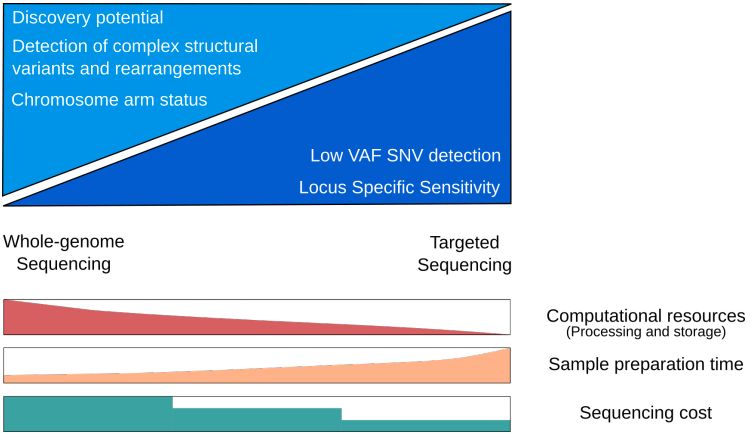
\includegraphics[width=0.6\linewidth]{wg.png}
        \caption{\label{fig:wg}Whole genome vs targeted sequencing}
    \end{figure}

    \subsection{Challenges in tracking tumour evolution with liquid biopsies}
    When tracking tumour evolution with liquid biopsies different parameters need to be considered:

    \begin{multicols}{2}
        \begin{itemize}
            \item ctDNA content: fraction of tumour content in circulation/
            \item Polyploidy: allelic imbalance events.
            \item The ability to detect signal is gene region dependent and individual dependent.
            \item Different metastasis have different DNA release rates.
        \end{itemize}
    \end{multicols}


        \subsubsection{An example of similarity between two plasma samples between two different tumours}
        Figure \ref{fig:challenges} depicts metastatic biopsy time points during clinical progression from CRPC-Adeno to CRPC-NE.
        Plasma sample at time of CRPCA-Adeno with lymph node and bone metastases displayed a genomic ctDNA profile similar to the one of CRPC-NE liver metastasis observed on imaging and biopsied $3$ months later at time of progression on abiraterone.

        \begin{figure}[H]
        \centering
            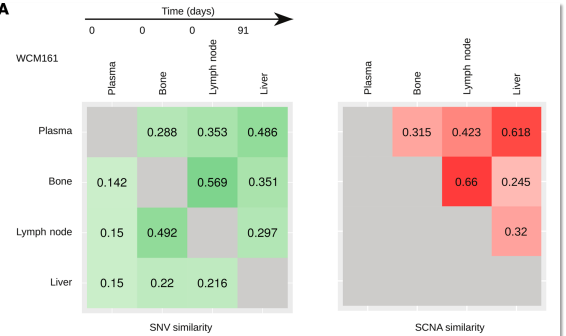
\includegraphics[width=0.7\linewidth]{time.png}
            \caption{Metastatic biopsy time points during clinical progression.}
        \label{fig:challenges}
        \end{figure}

\section{Interpretation of cell free DNA data}

    \subsection{Introduction}
    Interpretation of cell free DNA data from liquid biopsies poses a number of challenges to detect SNVs of the tumour fraction.

    \subsection{Normalization}
    When interpreting data from liquid biopsies, it is fundamental to contextualize a mutation after observing it.
    In order to associate a particular mutation to a particular diagnosis, the signal has to be normalized based on tumour content.
    Without normalization, tumour content is the most influential variable on the patient's prognosis and can mislead the analysis, making them useless.
    For example in figure \ref{fig:norm} depicts one mutation that is detected only in a specific type of tumour when it is actually present in other types too.
    It is not detected in other tumours because of the low tumour content of some samples.
    For this reason not all the literature available about liquid biopsies is reliable: lack of normalization leads to completely wrong conclusions.
    All assays that study cell-free DNA, from microarrays to extracellular vesicles need to be normalized.

    \begin{figure}[H]
    \centering
        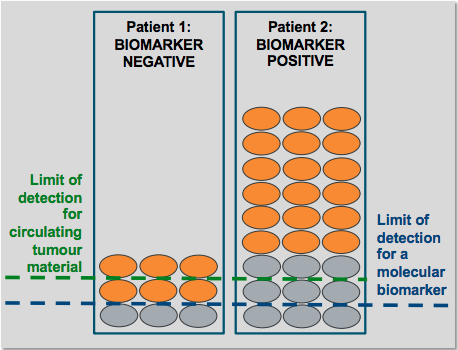
\includegraphics[width=0.4\linewidth]{norm.png}
        \caption{Two samples with the same percentage of tumour cells: the first one results negative for the marker because of its low tumour content.}
        \label{fig:norm}
    \end{figure}

    \subsection{Quantity of input material}
    Another source of errors in the interpretation of cfDNA data is the amount of input material: if the patient's tumour content is high, the results could be obtained with a limited amount of extracted nucleic acid, but if the tumour content is low, too little material can lower the chances of detecting tumour cells.
    This is visualized in figure \ref{fig:quan}, in which the same analyses are repeated with different quantities of starting material.
    It is visible that for a patient with high tumour content the results do not change even with as little as $5ng$ of cfDNA.

    \begin{figure}[H]
        \centering
        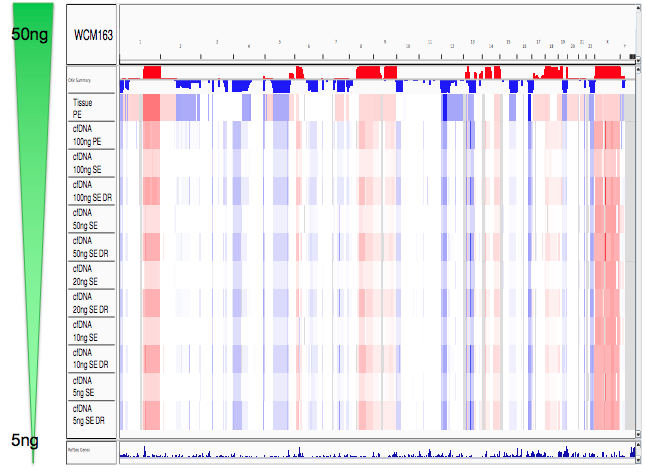
\includegraphics[width=0.5\linewidth]{quantity1.png}
        \caption{Change of resolution of analysis with different quantities of starting material.}
        \label{fig:quan}
    \end{figure}

    In most cases the tumour content is unknown before the analysis.
    This has to be taken into account when designing an experiment.
    Usually the standard procedure is to begin with $2ml$ of plasma, so the DNA obtained should be from $50 ng$ to $5ng$.
    For a pure sample $10ng$ of DNA should correspond to $\sim 1500$ diploid tumour genomes.
    In the case that no tumour is detected, the assay should be repeated with more material to be sure that the tumour is not present and not just undetected.
    Information about the patient state can guide the selection of the quantity of input material: for example, a patient in remission will require more material.
    Figure \ref{fig:quan2} depicts how copy number signal correlates well between different initial amounts of cfDNA for a sample with high tumour content.

    \begin{figure}[H]
        \centering
        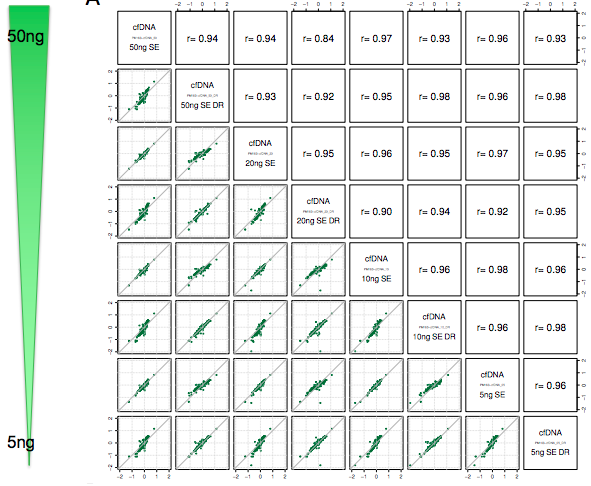
\includegraphics[width=0.7\linewidth]{quantity2.png}
        \caption{Correlation between copy number signal and initial amount of cfDNA for high tumour content.}
        \label{fig:quan2}
    \end{figure}

    \subsection{SNVs detection}
    Multiple tools are available to detect SNVs from liquid biopsies data.
    Each tool will probably give different results or partially concordant ones.
    Each tool can be tuned to favour some types of calls, so the tuning parameters should be carefully selected.
    SNVs detection in liquid biopsies faces different problems, both of technical and biological nature.

        \subsubsection{Technical problems}
        Technical problems that need to be addressed when detecting SNVs though liquid biopsies are:

        \begin{multicols}{2}
            \begin{itemize}
                \item PCR artefacts.
                \item Sequencing errors: one mutation should be validated by multiple reads to be confirmed.
                \item Problems related to the depth of coverage: the required coverage should be estimated considering the expected tumour content of the sample and deeper sequencing may be required.
            \end{itemize}
        \end{multicols}

        \subsubsection{Biological problems}
        Biological problems that need to be addressed when detecting SNVs though liquid biopsies are:

        \begin{multicols}{2}
            \begin{itemize}
                \item Low tumour content: ctDNA to cfDNA ratio.
                \item Clonal hematopoiesis: an hematopoietic stem cell starts making cells with the same genetic mutation.
                    To distinguish the signal coming from clonal hematopoiesis, it is compared with what has been sequenced before from solid tumours.
                    It is rare to observe something in liquid biopsy that has never been noticed in solid ones.
                \item Copy number variations and ploidy: with a whole genome duplication and a SNV only present on one allele, the signal corresponding to the mutation is only $25\%$ of what it should be and has to be correctly interpreted.
                \item Intra-patient tumour heterogeneity: very low allelic fractions for SNVs that are not clonal can be difficult to observe.
            \end{itemize}
        \end{multicols}


    \subsection{Two case studies}

        \subsubsection{Signal distribution in prostate cancer}
        In figure \ref{fig:case1} an assay to study specific signal distribution for prostate cancer is depicted.
        By analyzing this as a dynamic process, the overall distribution of clonal DNA can be derived.
        One of the lesion tracked was 21q22: the distribution on the top and the bottom are different at each time point with different dynamics.
        When the patient regressed 8p21, 21q22 emerged.

        \begin{figure}[H]
            \begin{tabular}{cc}
                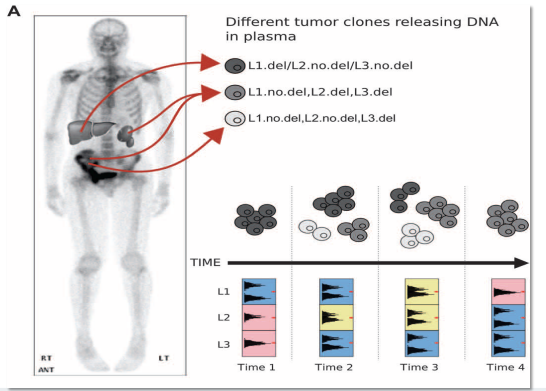
\includegraphics[width=0.4\linewidth]{case1a} &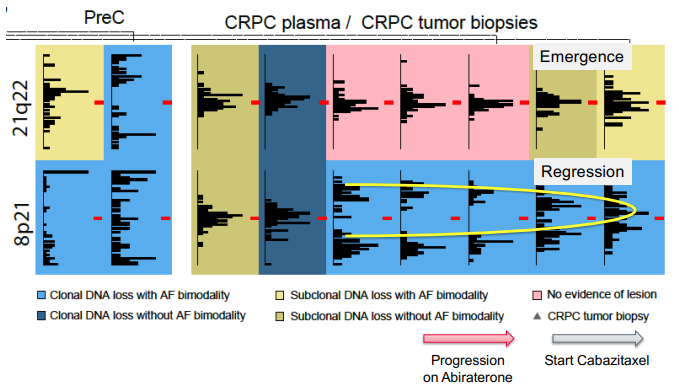
\includegraphics[width=0.6\linewidth]{case1b} \\
                (a)  & (b)  \\
            \end{tabular}
            \caption{\textbf{a)} Longitudinal sampling process. \textbf{b)} Emergence and progression of lesions over time.}
            \label{fig:case1}
        \end{figure}

        \subsubsection{Non-AR driven castration resistance prostate cancer}
        Non-AR driven castration resistant prostate cancer is really rare as a de novo disease, but it has a high rising incidence, especially after potent AR-pathway modifications.
        It is hard to treat and to diagnose.
        Both tissue and liquid biopsy analysis are performed to find:

        \begin{multicols}{2}
            \begin{itemize}
                \item Potential biomarkers for liquid biopsy.
                \item Distinguish the transition to severe stage.
            \end{itemize}
        \end{multicols}

        The first analysis from tissue biopsies sample allowed to investigate tumour heterogeneity, and determined the similarity of the metastasis.
        Homogeneity is higher for $NE$, the most aggressive phenotype.
        The same was observed in liquid biopsies, confirming the potential of the use of $NE$ biomarkers.
        A liquid biopsy reported equal result to a lymph node metastasis, with a clear signal.
        In other patients, certain genes switch from one cluster to another from tissue to plasma, suggesting that the metastatic representation was partially heterogeneous.
        It is clear how liquid biopsies provide a landscape overview.

        \begin{figure}[H]
        \centering
            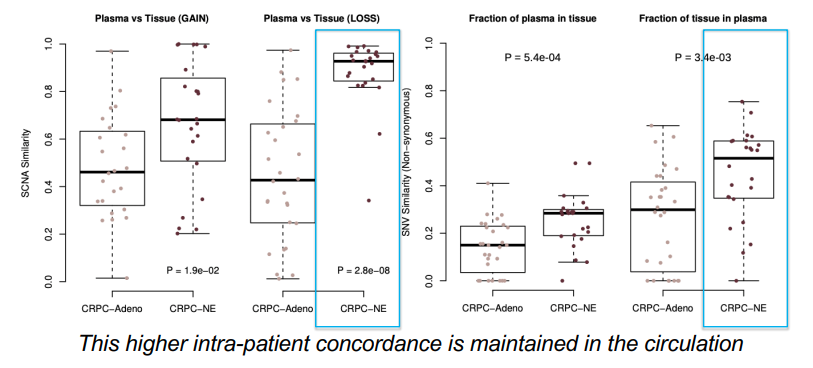
\includegraphics[width=0.7\linewidth]{case2.png}
            \caption{Concordance between two patients}
            \label{fig:case2}
        \end{figure}

        Figure \ref{fig:case2} depicts SCNA and SNV similarity for a man initially diagnosed with adenocarcinoma.
        The diagnosis switched to NE after clinical assessment.
        Plasma sample come before NE diagnosis and multiple tissue biopsies were performed.
        It was noted that the liver metastasis NE had lesion represented in the plasma sample, suggesting that a clone that was transforming was already present in the past.
        This makes clear how in certain cases, a liquid biopsy can be informative of something that would only emerge later clinically.
        Comparing the genomic content of each metastasis with the data coming from a liquid biopsy, a measure of the modification contributing more to the disease can be obtained.
